% =============================================================================
%  Into Frame -- slide deck (Beamer)
%
%  Build:  pdflatex slides.tex
%
%  A PDF twin of Into-Frame-slides.pptx, for machines without PowerPoint.
%  Figures are shared with the report, so both stay in step.
% =============================================================================
\documentclass[aspectratio=169,11pt]{beamer}

\usepackage[T1]{fontenc}
\usepackage[utf8]{inputenc}
\usepackage{lmodern}
\usepackage{graphicx}
\usepackage{siunitx}
\usepackage{booktabs}
\usepackage{xcolor}

\graphicspath{{figures/}}

% ---- a plain, quiet theme ---------------------------------------------------
\usetheme{default}
\usecolortheme{default}
\setbeamertemplate{navigation symbols}{}
\setbeamertemplate{itemize items}[circle]

\definecolor{ink}{HTML}{1A1A1A}
\definecolor{muted}{HTML}{666666}
\definecolor{accent}{HTML}{1F77B4}
\definecolor{warn}{HTML}{C0501E}

\setbeamercolor{normal text}{fg=ink}
\setbeamercolor{frametitle}{fg=ink}
\setbeamercolor{itemize item}{fg=accent}
\setbeamercolor{itemize subitem}{fg=accent}
\setbeamerfont{frametitle}{size=\Large,series=\bfseries}
\setbeamertemplate{frametitle}{%
  \vspace{0.6em}\hspace{0.2em}\insertframetitle\par\vspace{-0.2em}}
\setbeamertemplate{footline}{%
  \hfill\color{muted}\scriptsize\insertframenumber\hspace{1.2em}\vspace{0.5em}}

\newcommand{\kicker}[1]{{\color{accent}\bfseries\scriptsize\MakeUppercase{#1}}\par\vspace{0.2em}}
\newcommand{\lead}[1]{{\color{ink}\bfseries #1}}
\newcommand{\quietx}[1]{{\color{muted}#1}}
\newcommand{\flag}[1]{{\color{warn}\bfseries #1}}

\begin{document}

% 1 --------------------------------------------------------------------------
{\setbeamertemplate{footline}{}
\begin{frame}[plain]
  \vspace{0.6em}
  {\Huge\bfseries Jumping Into the Frame}\par\vspace{0.6em}
  {\large\color{muted} Reconstructing Interactive, Physically-Grounded 3D
   Environments from a Single Image}\par\vspace{0.9em}
  {\small\color{muted} Joshua Ford \quad\textperiodcentered\quad Advisor: Marie-Paule Cani}
  \vfill
  \noindent\makebox[\textwidth]{%
    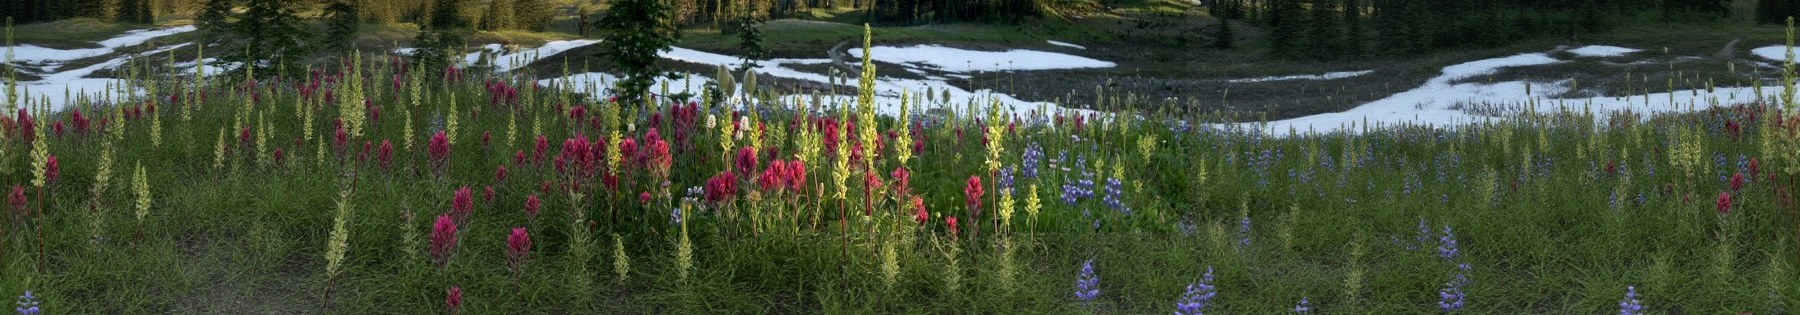
\includegraphics[width=\paperwidth,height=0.30\paperheight]{rainier/panorama-band.jpg}}
\end{frame}}

% 2 --------------------------------------------------------------------------
\begin{frame}{A photograph is not a place}
  \kicker{motivation}
  \begin{columns}[T]
    \begin{column}{0.54\textwidth}
      \small
      \begin{itemize}\setlength\itemsep{0.7em}
        \item Recovering 3D from one view is underconstrained: infinitely many
              scenes project to the same image.
        \item People read a photograph as a place anyway --- the ground continues
              past the frame, the occluded side of a rock exists, the flowers are
              individual plants.
        \item Photographs are among the most abundant records of place we have.
        \item The goal: an environment you can \emph{jump into}, not a picture you
              can orbit.
      \end{itemize}
    \end{column}
    \begin{column}{0.44\textwidth}
      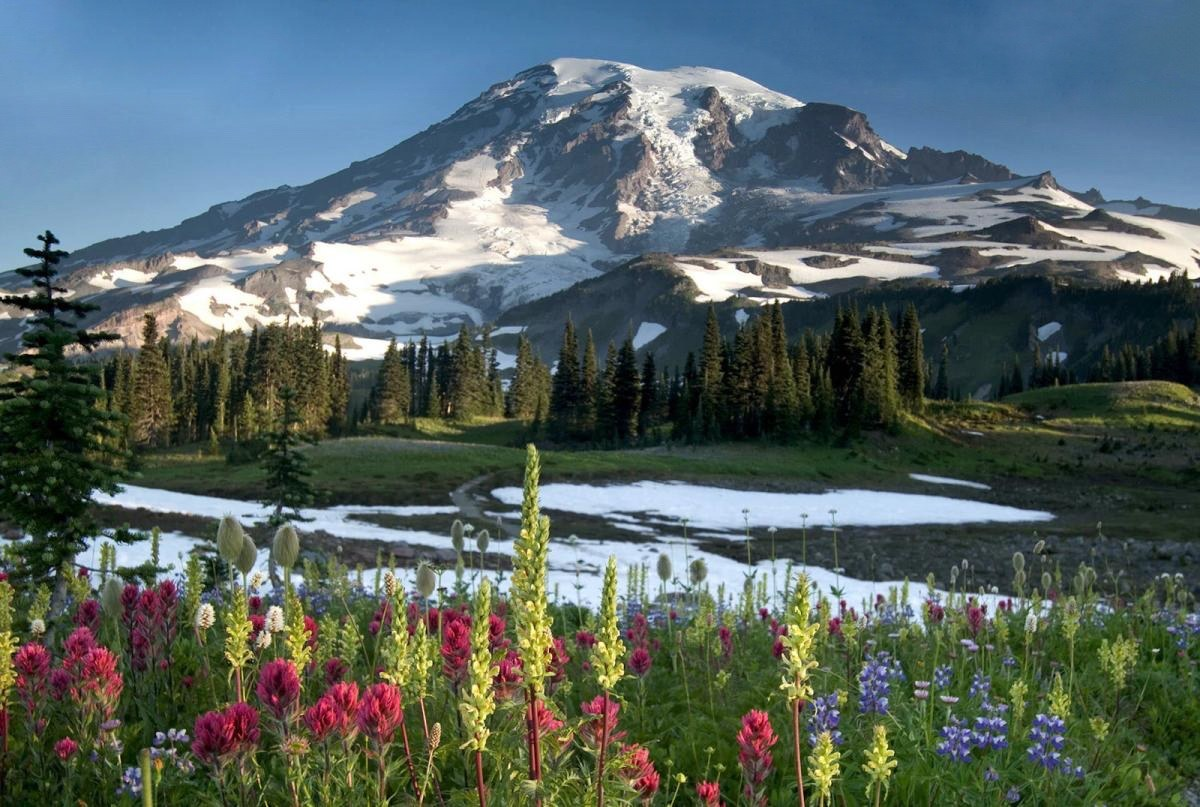
\includegraphics[width=\linewidth]{rainier/input.jpg}
    \end{column}
  \end{columns}
\end{frame}

% 3 --------------------------------------------------------------------------
\begin{frame}{Four problems that compound}
  \kicker{the challenge}
  \small
  \begin{itemize}\setlength\itemsep{0.85em}
    \item \lead{Extreme ill-posedness.} \quietx{Roughly $5/6$ of the sphere is never
          observed, and everything behind every foreground object is unknown.}
    \item \lead{Compounding error.} \quietx{Depth, then geometry, then materials,
          then objects. A discrepancy invisible at one stage is structural by the next.}
    \item \lead{Heterogeneous content.} \quietx{A height field suits a mountainside,
          a mesh a tree, a scattered population a meadow, an animated surface the
          sea --- and they must share one coordinate frame, scale and lighting.}
    \item \lead{Interactivity budget.} \quietx{Stereo rendering at headset frame
          rates constrains every choice, hardest on the animated elements that
          make it interactive.}
  \end{itemize}
\end{frame}

% 4 --------------------------------------------------------------------------
\begin{frame}{Prior work stops at viewable}
  \kicker{related work}
  \small
  \begin{itemize}\setlength\itemsep{0.7em}
    \item Single-image scene generation has advanced fast: CubeDiff, DreamCube,
          PanoDreamer, LayerPano3D, WorldGen, SphericalDreamer.
    \item These optimize visual fidelity from viewpoints near the original camera.
    \item The output is a panorama, a layered mesh, or a radiance field ---
          something to look at.
  \end{itemize}
  \vspace{1.2em}
  \flag{What none of them return: a collidable surface, a population whose density
  can be sampled, a water plane separable from its bed, or a mesh with a skeleton in it.}
\end{frame}

% 5 --------------------------------------------------------------------------
\begin{frame}{One idea: reconstruct by physical role}
  \kicker{approach}
  \small
  A scene is not one thing. Ground, discrete objects, ground cover, water and sky
  differ in how they must be reconstructed, represented, textured, and how they
  behave at runtime.
  \vspace{0.7em}
  \begin{itemize}\setlength\itemsep{0.45em}
    \item \lead{Terrain} \quietx{--- a continuous height field carrying collision}
    \item \lead{Objects} \quietx{--- meshes reconstructed once per appearance group, then instanced}
    \item \lead{Ground cover} \quietx{--- a scattered population, too numerous to place individually}
    \item \lead{Water} \quietx{--- a separate leveled surface with an animated shader}
    \item \lead{Motion} \quietx{--- rigid bodies or anchored sway, per object}
    \item \lead{Sky} \quietx{--- skybox and image-based lighting source}
  \end{itemize}
\end{frame}

% 6 --------------------------------------------------------------------------
\begin{frame}{The pipeline}
  \kicker{42 stages, 38 active}
  \vspace{-0.3em}
  \centering
  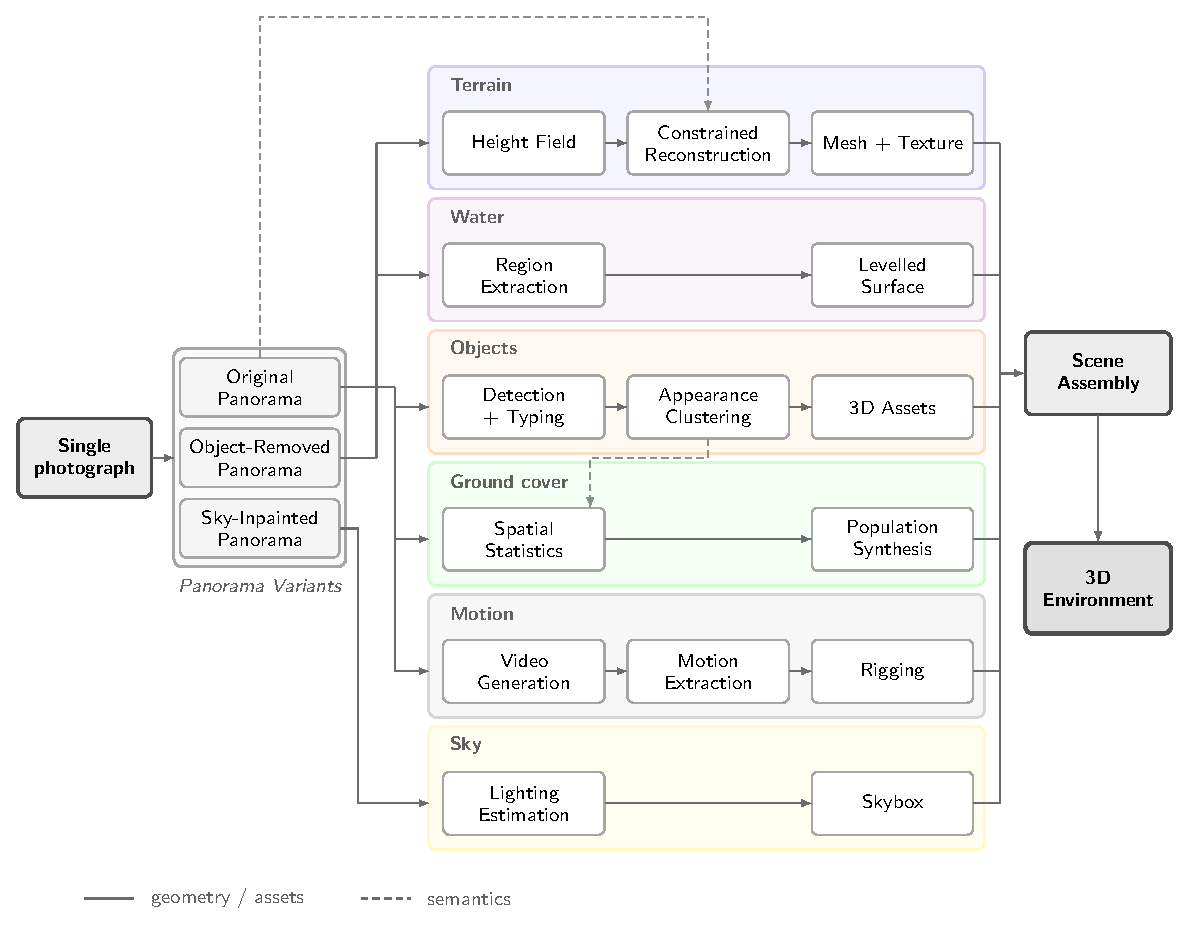
\includegraphics[height=0.78\textheight]{pipeline-current.png}
\end{frame}

% 7 --------------------------------------------------------------------------
\begin{frame}{One photograph becomes a sphere}
  \kicker{the panoramic substrate}
  \begin{columns}[T]
    \begin{column}{0.32\textwidth}
      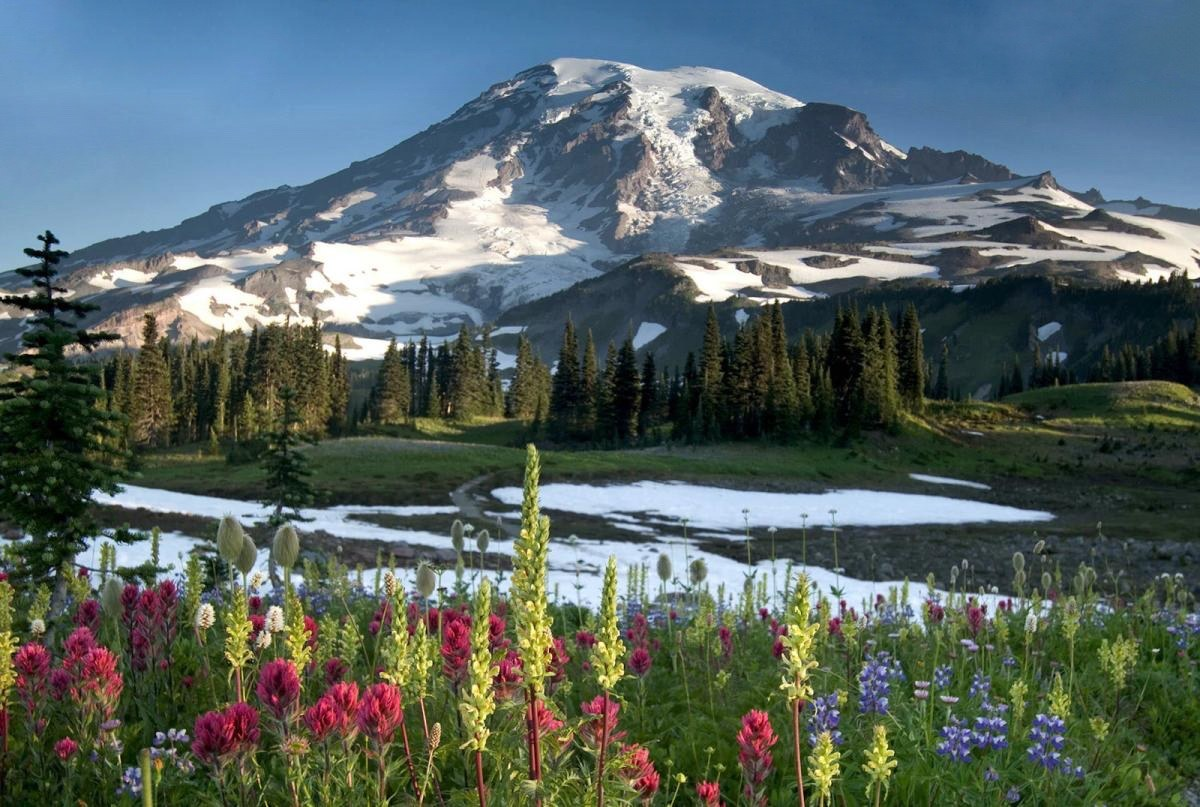
\includegraphics[width=\linewidth]{rainier/input.jpg}\\[0.3em]
      {\scriptsize\color{muted} Input: about a sixth of the sphere}
    \end{column}
    \begin{column}{0.64\textwidth}
      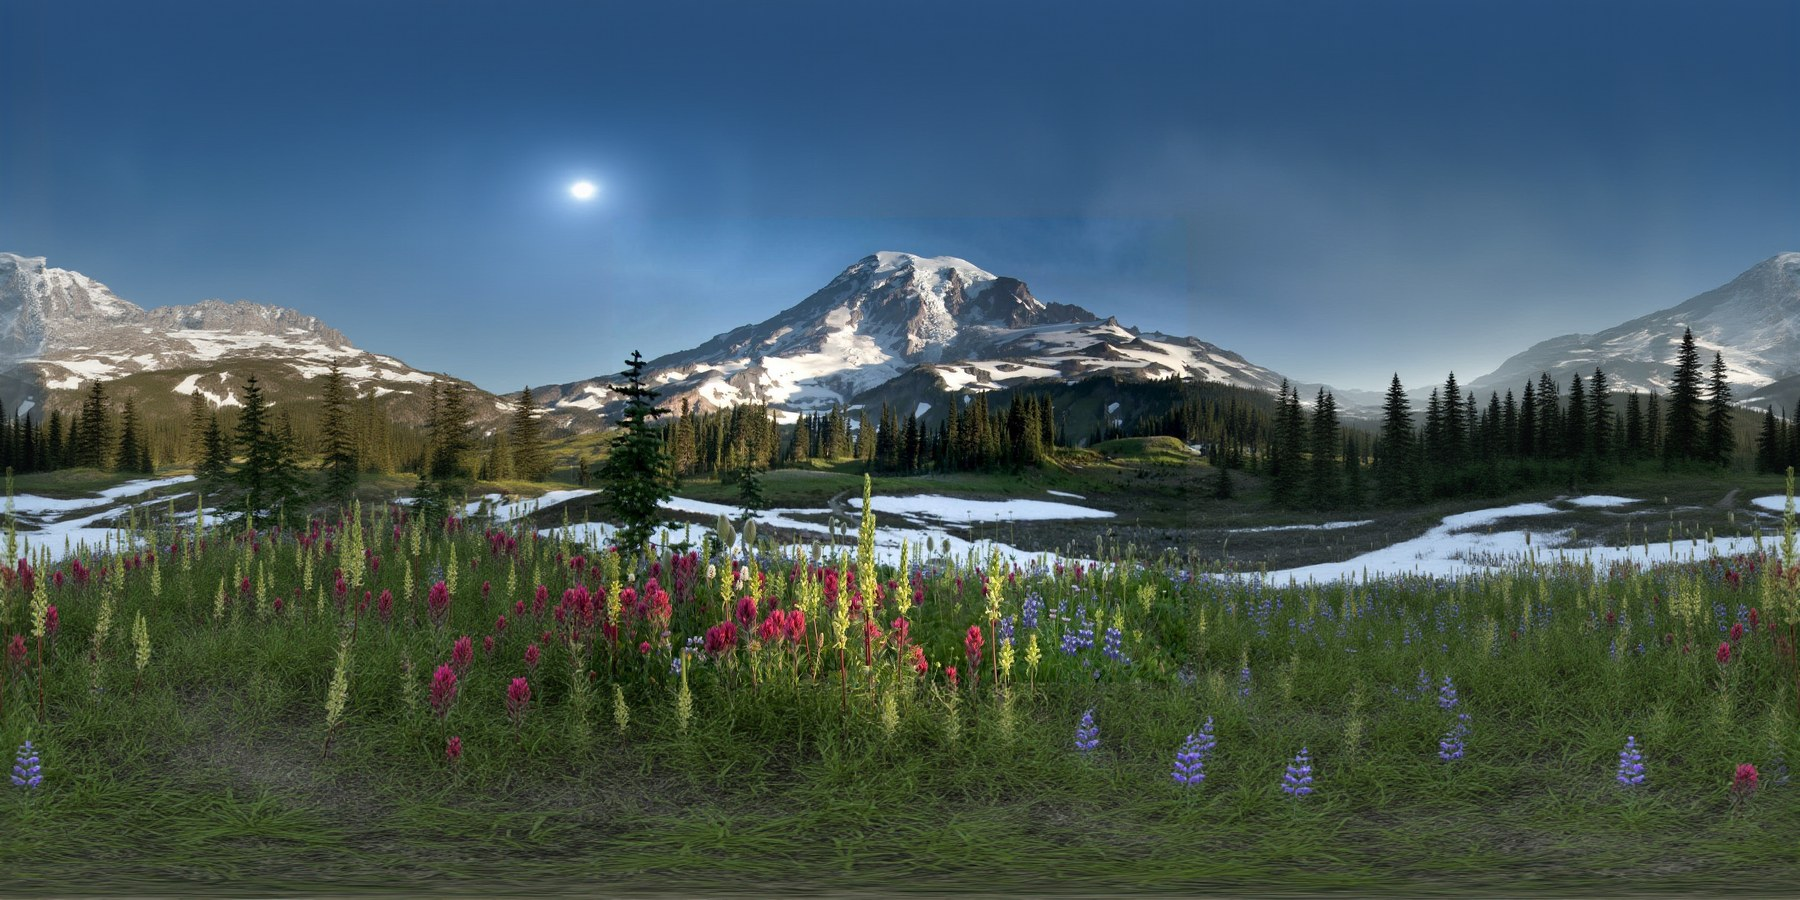
\includegraphics[width=\linewidth]{rainier/panorama.jpg}\\[0.3em]
      {\scriptsize\color{muted} Generated panorama: the other ${\sim}83\%$ is synthesized}
    \end{column}
  \end{columns}
  \vspace{0.4em}
  \footnotesize
  \begin{itemize}\setlength\itemsep{0.25em}
    \item WorldGen by default; FLUX, CubeDiff and DreamCube are interchangeable backends.
    \item The panorama is an intermediate representation, not the deliverable.
  \end{itemize}
\end{frame}

% 8 --------------------------------------------------------------------------
\begin{frame}{Depth is relative --- calibration makes it metric}
  \kicker{the panoramic substrate}
  \begin{columns}[T]
    \begin{column}{0.56\textwidth}
      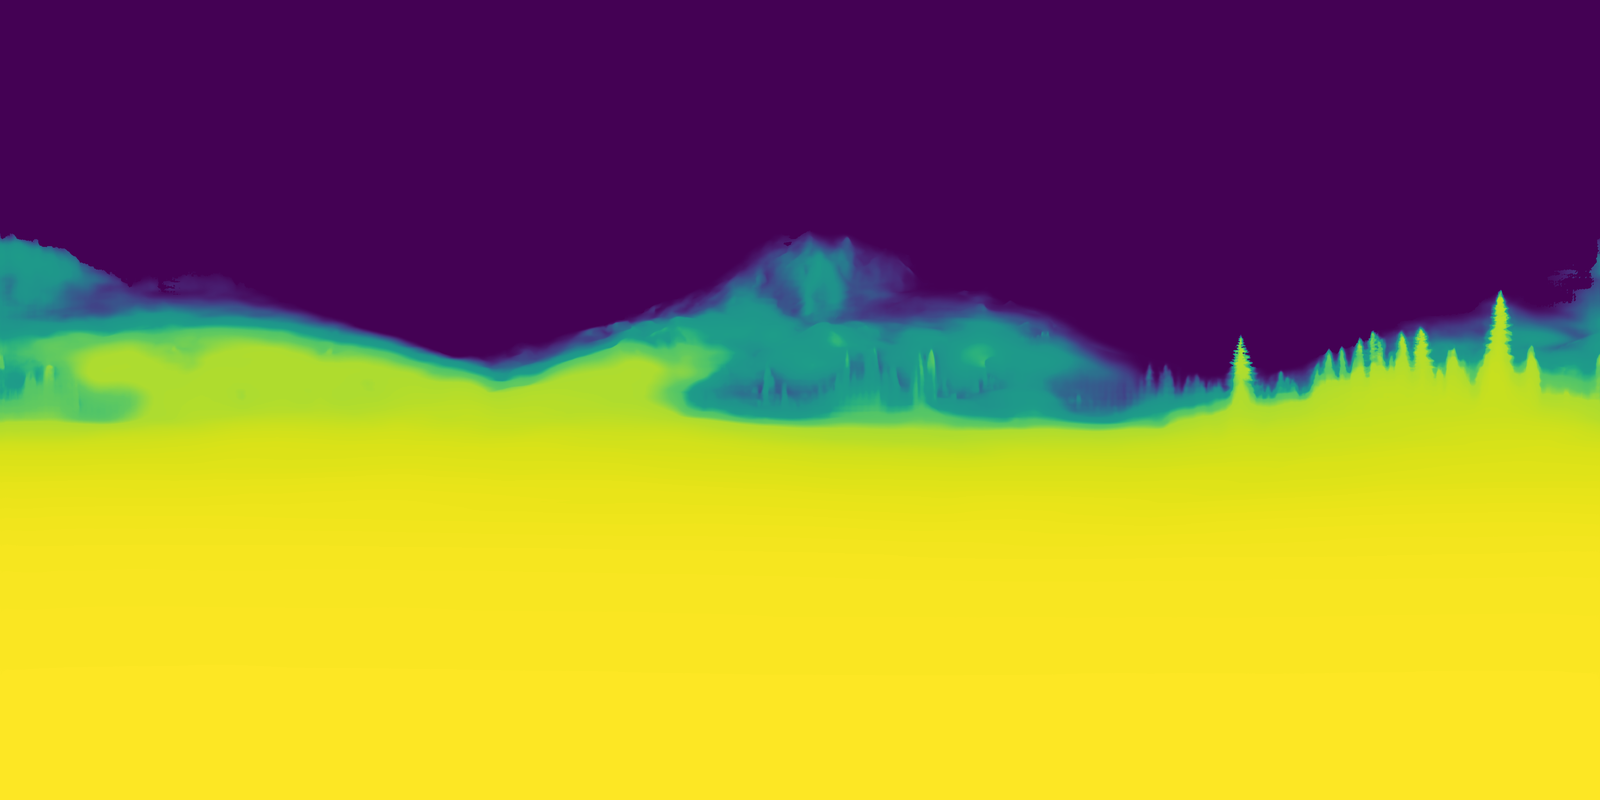
\includegraphics[width=\linewidth]{rainier/depth-calibrated.png}
    \end{column}
    \begin{column}{0.42\textwidth}
      \scriptsize
      \begin{itemize}\setlength\itemsep{0.55em}
        \item Panoramic depth is relative. We fit a monotonic curve against
              Depth Anything~3 on the original photo, over the region it observed.
        \item 14 quantile bins, median knots, running-maximum monotonicity.
        \item Beyond the fitted range we extrapolate in log-depth, capped at $20\times$.
      \end{itemize}
    \end{column}
  \end{columns}
  \vspace{0.9em}
  \small
  \flag{Angularly faithful but metrically compressed.} \quietx{Near distances are
  accurate, far ones systematically shrunk --- and object size, computed as angular
  extent times depth, inherits that shrinkage eight stages later.}
\end{frame}

% 9 --------------------------------------------------------------------------
\begin{frame}{Two panoramas, because they answer different questions}
  \kicker{the panoramic substrate}
  \centering
  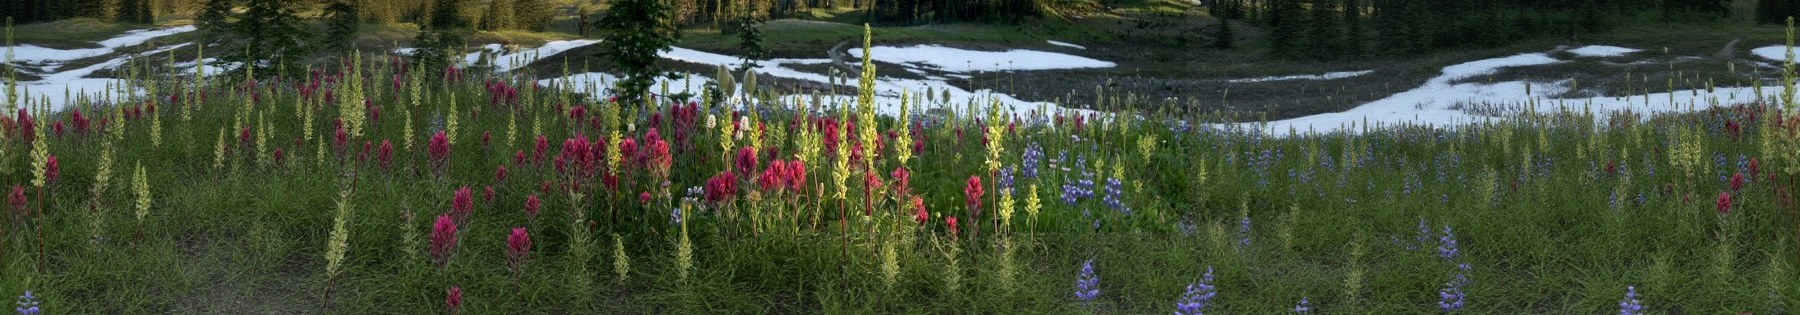
\includegraphics[width=0.92\linewidth]{rainier/panorama-band.jpg}\\[0.15em]
  {\scriptsize\color{muted} Original --- what the scene contains}\\[0.5em]
  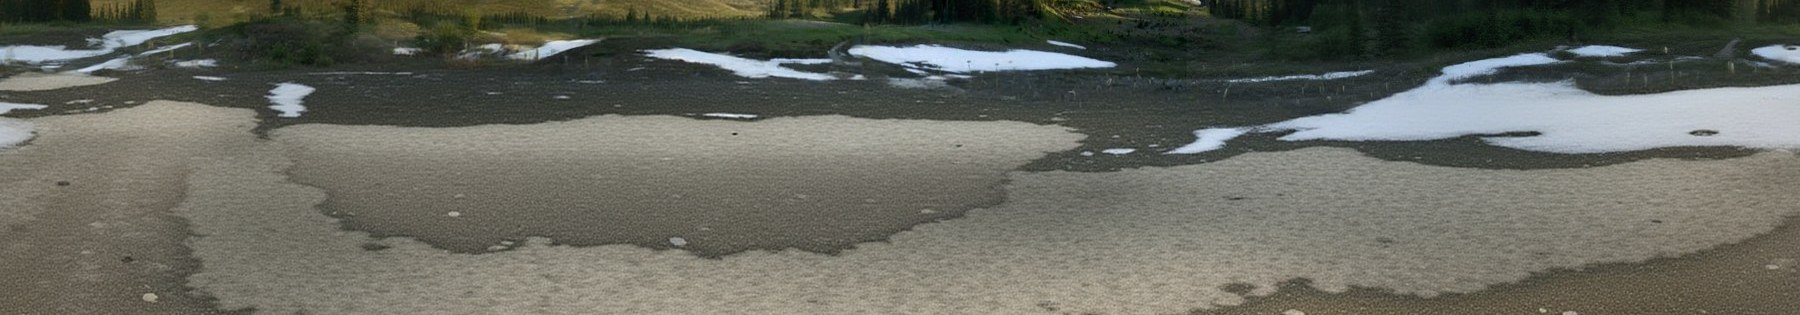
\includegraphics[width=0.92\linewidth]{rainier/panorama-object-removed-band.jpg}\\[0.15em]
  {\scriptsize\color{muted} Object-removed --- what the ground looks like}
  \vspace{0.4em}
  \par\raggedright\footnotesize
  Depth from the original would place the flower canopy, not the ground, at the
  bottom of the height field. Geometry reads the object-removed panorama;
  semantics reads the original.
\end{frame}

% 10 -------------------------------------------------------------------------
\begin{frame}{Completing terrain that was never seen}
  \kicker{terrain geometry}
  \centering
  \begin{columns}[T]
    \begin{column}{0.31\textwidth}\centering
      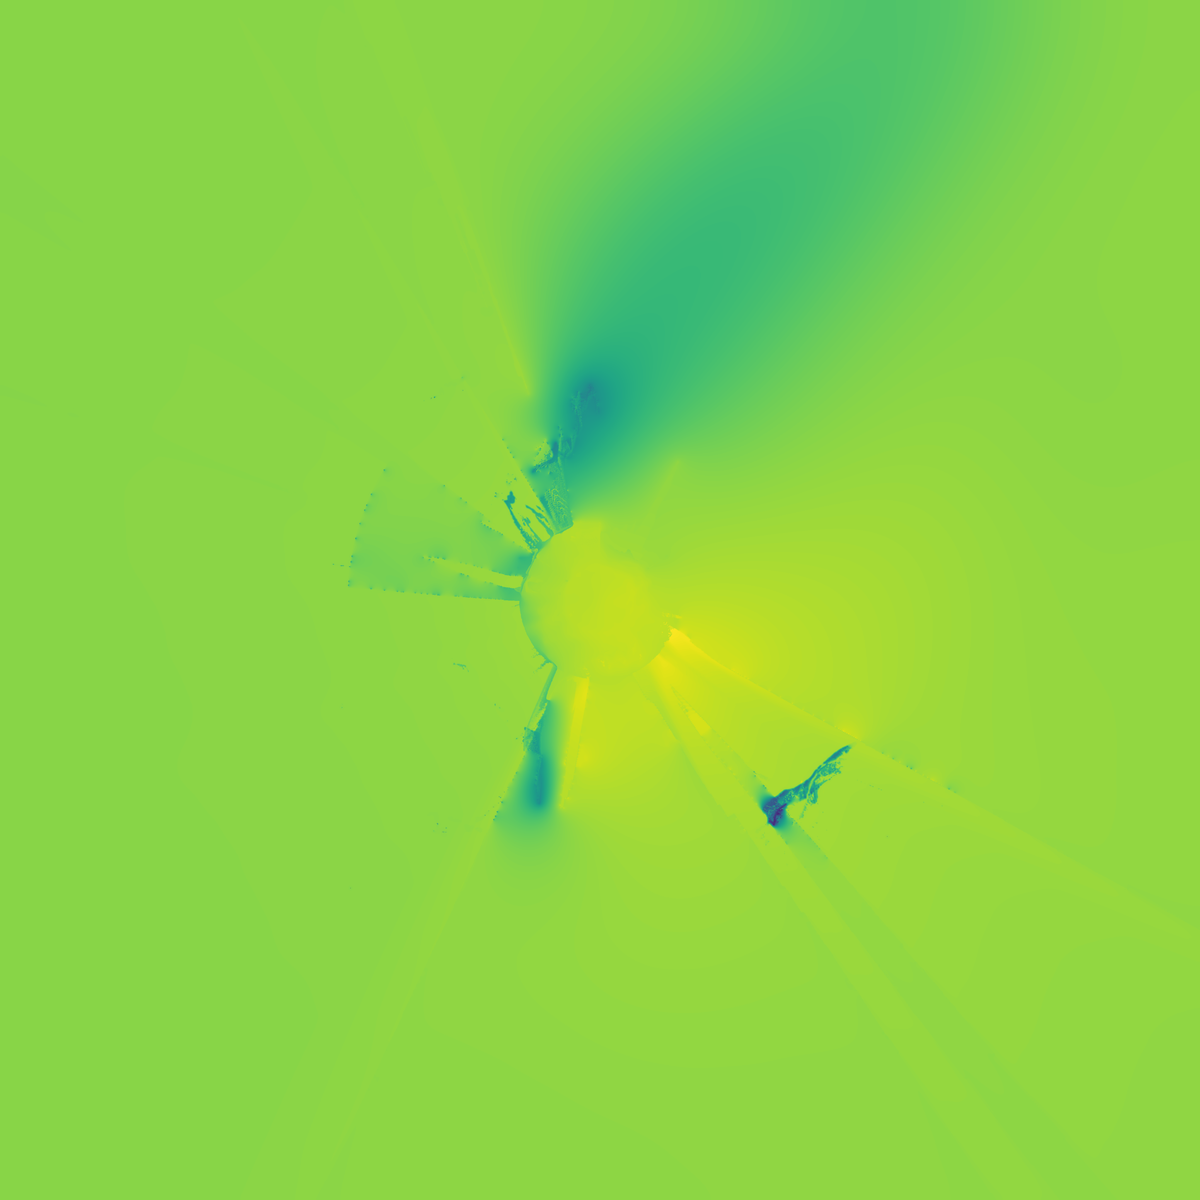
\includegraphics[width=\linewidth]{rainier/heightmap-observed.png}\\[0.25em]
      {\scriptsize\color{muted} Projected observations --- $7\%$ of the grid}
    \end{column}
    \begin{column}{0.31\textwidth}\centering
      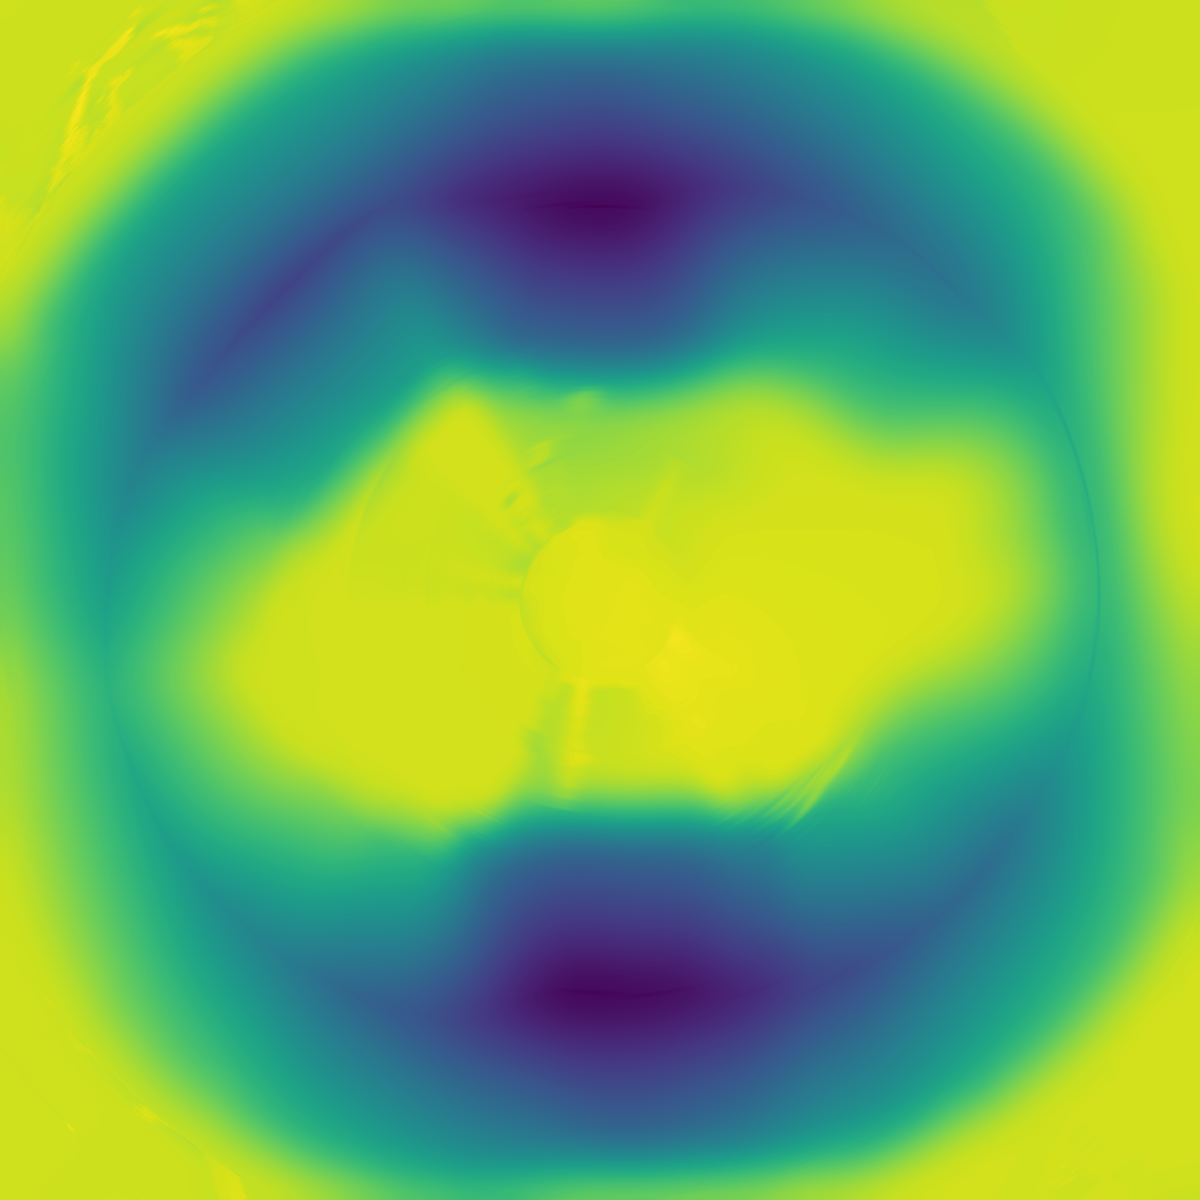
\includegraphics[width=\linewidth]{rainier/heightmap-reconstructed.png}\\[0.25em]
      {\scriptsize\color{muted} Harmonic completion}
    \end{column}
    \begin{column}{0.31\textwidth}\centering
      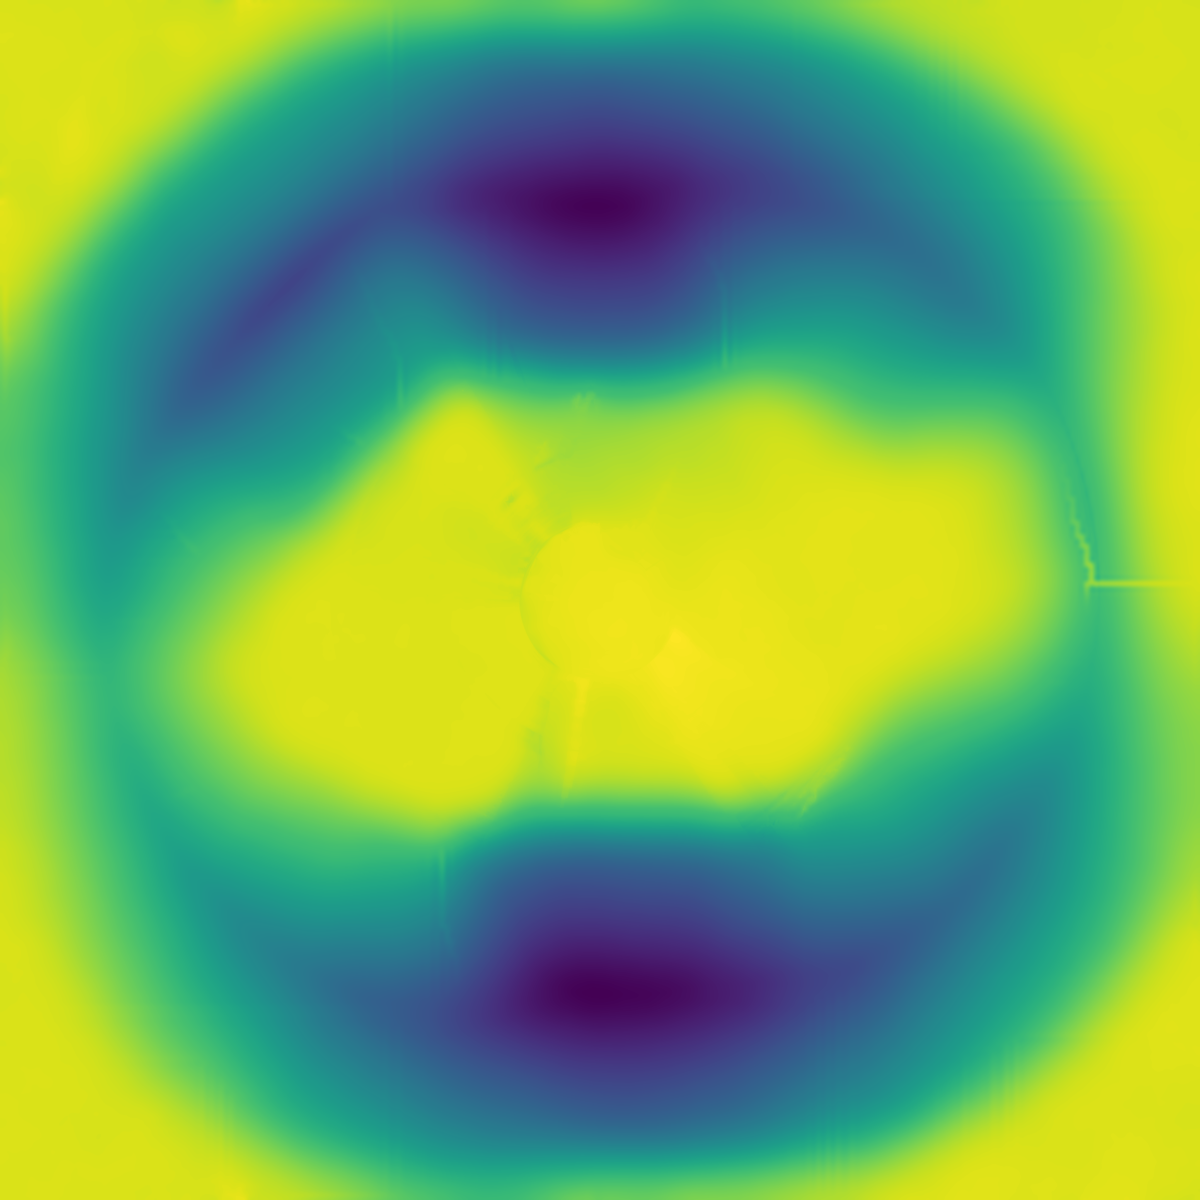
\includegraphics[width=\linewidth]{rainier/heightmap-eroded.png}\\[0.25em]
      {\scriptsize\color{muted} Fluvial erosion}
    \end{column}
  \end{columns}
  \vspace{0.3em}
  \par\raggedright\scriptsize
  Measured cells become Dirichlet boundary conditions and are never modified. The
  unknown region is the smoothest surface consistent with them --- then Landlab's
  fluvial incision gives it drainage structure, so invented relief is shaped by the
  process that shapes real landscapes.
\end{frame}

% 11 -------------------------------------------------------------------------
\begin{frame}{The sky boundary is assumed to be ground}
  \kicker{terrain --- the key assumption}
  \begin{columns}[T]
    \begin{column}{0.46\textwidth}
      \small
      \begin{itemize}\setlength\itemsep{0.6em}
        \item Past a few hundred meters the depth model has saturated. The
              silhouette is the only signal left.
        \item For each panorama column, the first non-sky pixel gives an elevation
              angle, placed at a fixed radius.
        \item This works whenever the horizon really is a landform.
      \end{itemize}
      \vspace{0.8em}
      \flag{In Paris the horizon is a roofline \SI{40}{\meter} away. A flat height
      field (\SI{-6.0}{\meter} to \SI{-0.2}{\meter}) became \SI{-13.1}{\meter} to
      \SI{+70.9}{\meter} --- a hill on the cathedral.}
    \end{column}
    \begin{column}{0.52\textwidth}
      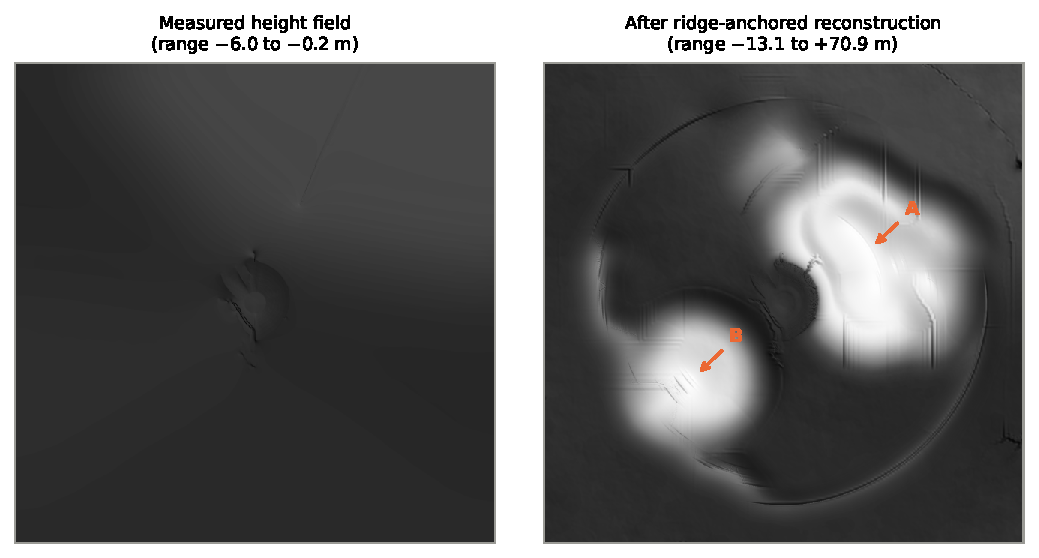
\includegraphics[width=\linewidth]{paris-terrain.pdf}\\[0.3em]
      {\scriptsize\color{muted} Paris height field: measured (left) vs after
       ridge-anchored reconstruction (right)}
    \end{column}
  \end{columns}
\end{frame}

% 12 -------------------------------------------------------------------------
\begin{frame}{Projecting the photo onto the ground fails}
  \kicker{terrain appearance}
  \begin{columns}[T]
    \begin{column}{0.38\textwidth}
      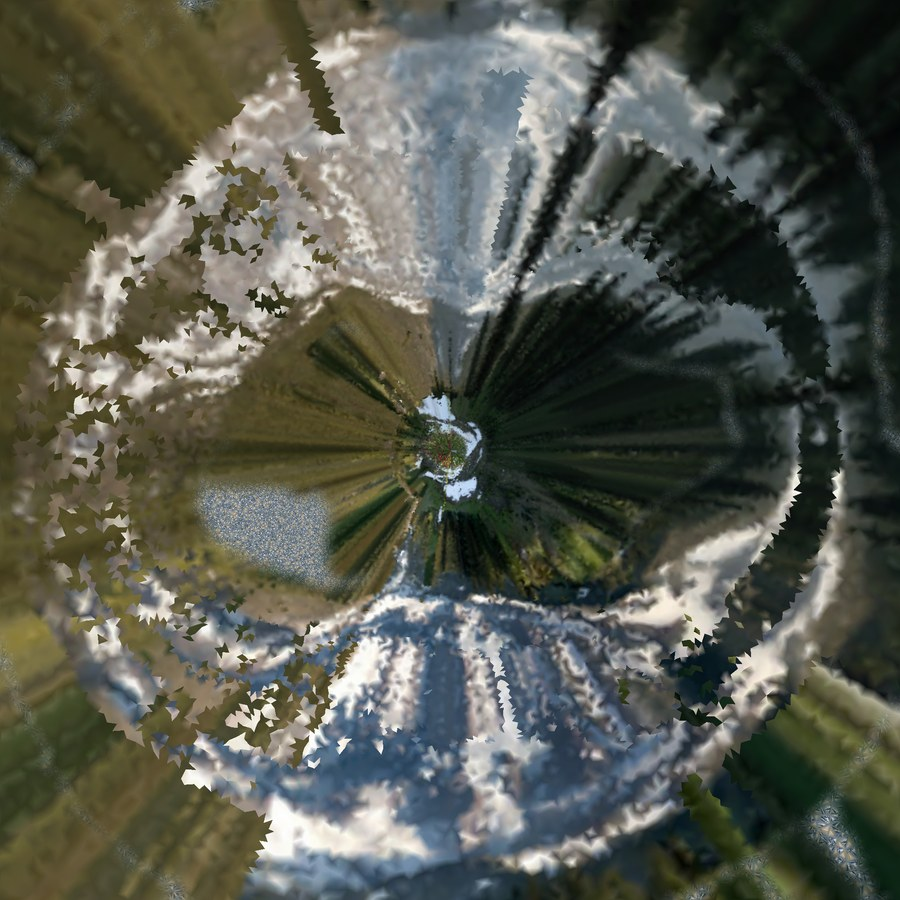
\includegraphics[width=\linewidth]{rainier/tile-terrain.jpg}
    \end{column}
    \begin{column}{0.60\textwidth}
      \small
      \begin{itemize}\setlength\itemsep{0.7em}
        \item \lead{Grazing incidence.} \quietx{At \SI{80}{\meter} one panorama row
              covers roughly \SI{12}{\meter} of ground. The result is radial smearing.}
        \item \lead{Upright content.} \quietx{A \SI{0.5}{\meter} flower spans a range
              of elevations, each landing at a different radius --- one flower
              becomes a streak meters long.}
        \item \lead{The fix.} \quietx{A layered splat material: real photographic
              color where projection is trustworthy, pattern-textured real material
              where it is not, generated tiles only as a last resort.}
      \end{itemize}
    \end{column}
  \end{columns}
\end{frame}

% 13 -------------------------------------------------------------------------
\begin{frame}{Detect, cluster, reconstruct once, instance everywhere}
  \kicker{object decomposition}
  \centering
  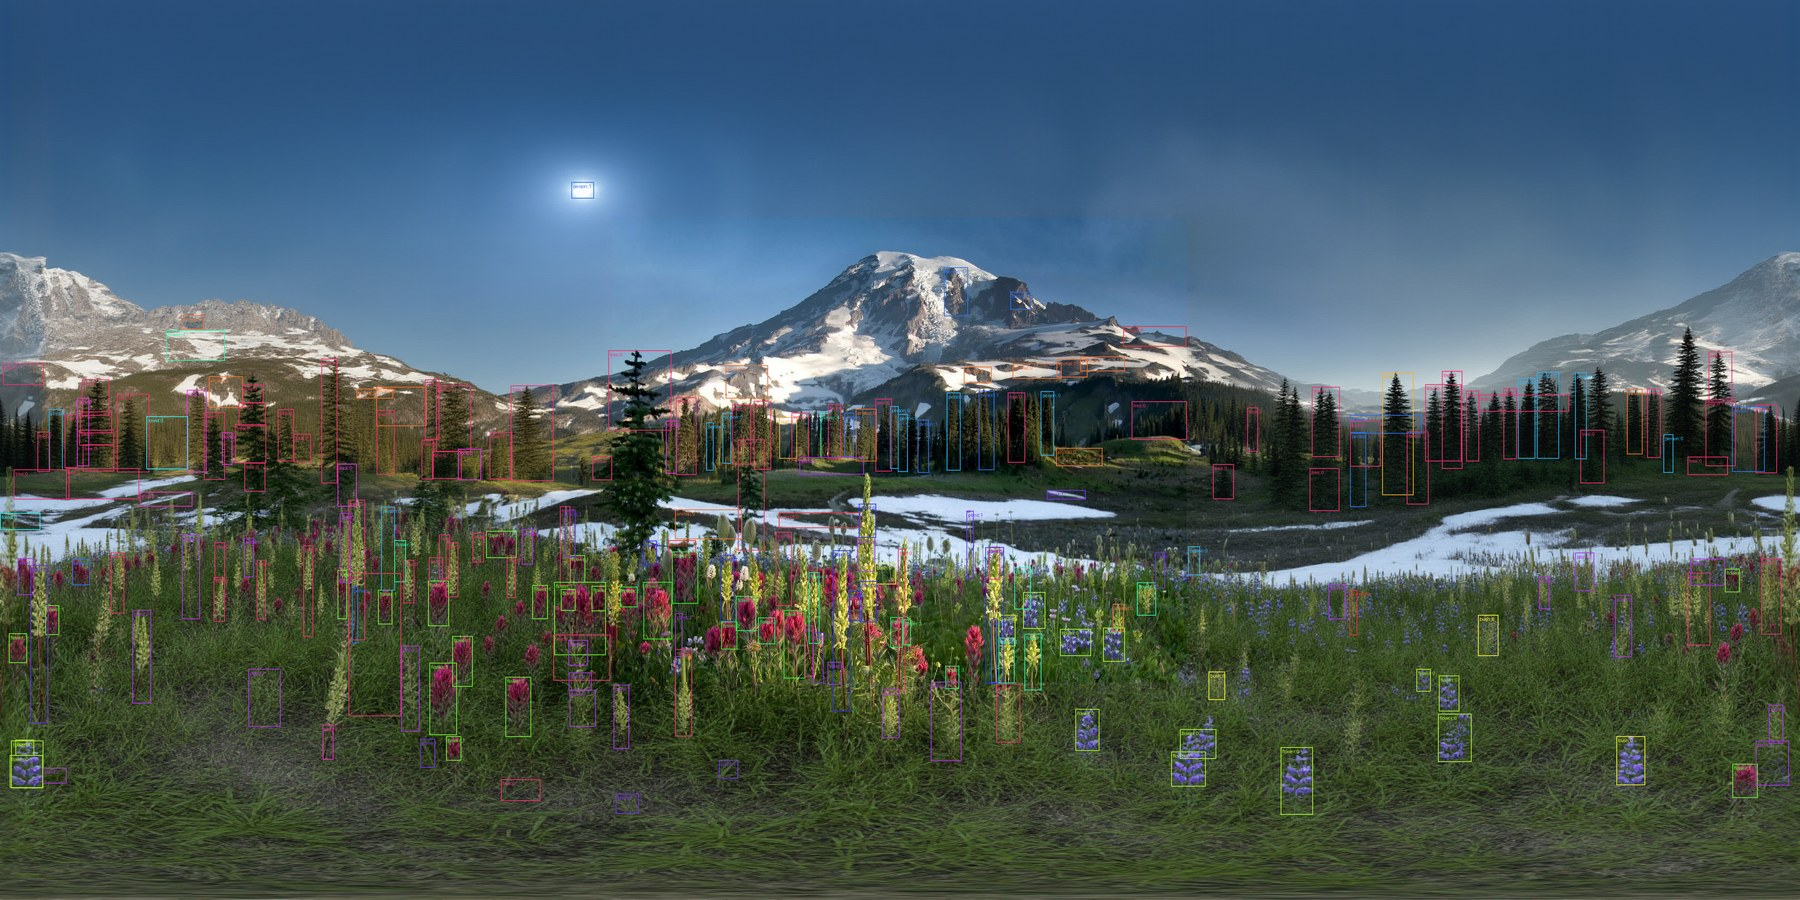
\includegraphics[width=0.60\linewidth]{rainier/clusters.jpg}
  \vspace{0.3em}
  \par\raggedright\scriptsize
  \begin{itemize}\setlength\itemsep{0.4em}
    \item SAM~2 segments the full $360^\circ$; CLIP classifies; Grounding DINO
          verifies by having to \emph{find} the label in the crop.
    \item DINOv2 sub-clusters each class into appearance variants. One mesh per
          (class, bucket) group, instanced at every member.
    \item \lead{Three representations:} \quietx{reconstructed mesh $\rightarrow$
          crossed card (three fixed planes) $\rightarrow$ camera-facing billboard,
          chosen on projected angular size.}
  \end{itemize}
\end{frame}

% 14 -------------------------------------------------------------------------
\begin{frame}{A detector finds tens of flowers in a meadow of thousands}
  \kicker{population synthesis}
  \begin{columns}[T]
    \begin{column}{0.34\textwidth}\centering
      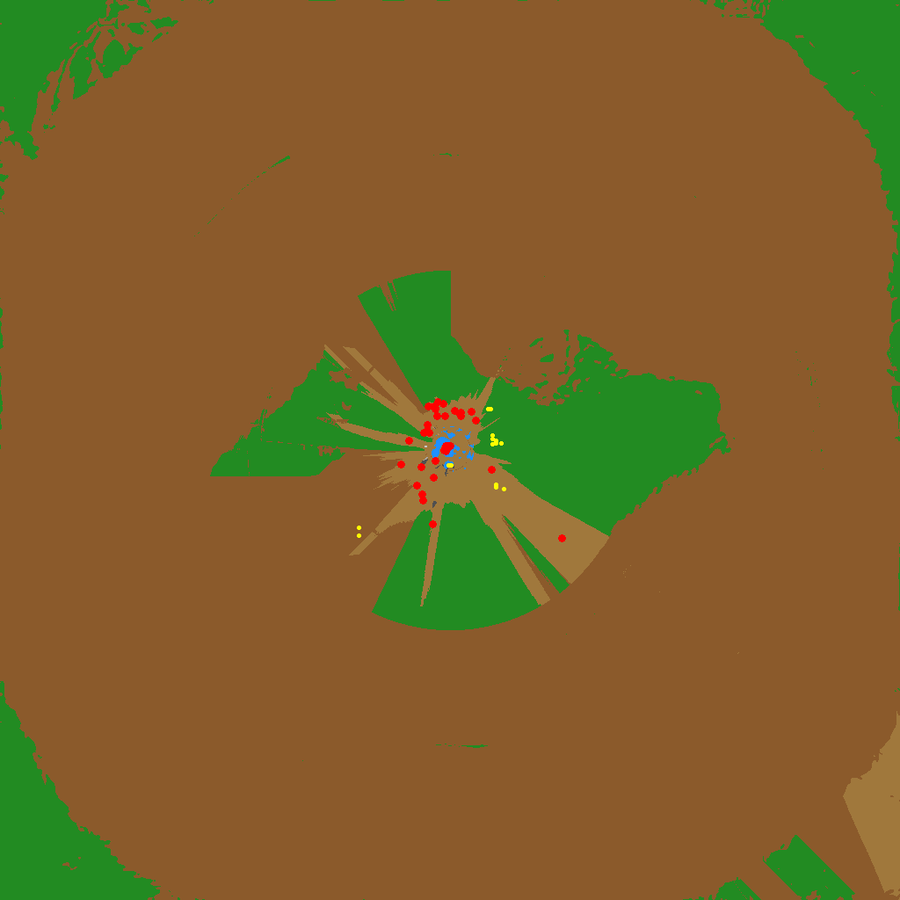
\includegraphics[width=0.86\linewidth]{rainier/synthesis-tree.png}\\[0.25em]
      {\scriptsize\color{muted} Synthesized tree population}
    \end{column}
    \begin{column}{0.34\textwidth}\centering
      
\includegraphics[width=0.86\linewidth]{rainier/grass-area.png}\\[0.25em]
      {\scriptsize\color{muted} Ground-cover mask}
    \end{column}
    \begin{column}{0.30\textwidth}
      \scriptsize
      \begin{itemize}\setlength\itemsep{0.6em}
        \item \lead{Synthesis} \quietx{matches the pair-correlation statistics of real
              detections --- a point process, not a fixed density.}
        \item \lead{Ground cover} \quietx{has no discrete instances to generalize from.
              It is scattered over a mask, vetoed by excess-green so snowfields do
              not become meadow.}
      \end{itemize}
    \end{column}
  \end{columns}
\end{frame}

% 15 -------------------------------------------------------------------------
\begin{frame}{Estimate the light, then remove it from every asset}
  \kicker{lighting}
  \begin{columns}[T]
    \begin{column}{0.40\textwidth}\centering
      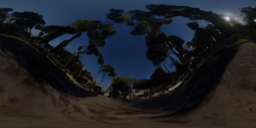
\includegraphics[width=\linewidth]{rainier/lighting-log.png}\\[0.3em]
      {\scriptsize\color{muted} Estimated HDR environment (log scale)}
    \end{column}
    \begin{column}{0.58\textwidth}
      \small
      \begin{itemize}\setlength\itemsep{0.6em}
        \item LuxDiT recovers an HDR environment and a dominant light direction.
        \item Every asset is cut from a photograph, so it already carries the light
              of the moment it was taken.
        \item IntrinsicDiffusion separates albedo from shading, so the client
              relights material color rather than a photograph.
        \item This is what makes assets portable: an instance rarely sits where it
              was photographed.
      \end{itemize}
    \end{column}
  \end{columns}
\end{frame}

% 16 -------------------------------------------------------------------------
\begin{frame}{Motion from a generated video}
  \kicker{animation}
  \begin{columns}[T]
    \begin{column}{0.40\textwidth}\centering
      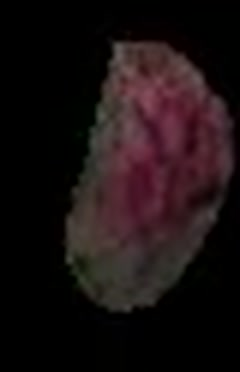
\includegraphics[width=0.21\linewidth]{rainier/motion-26.jpg}\hfill
      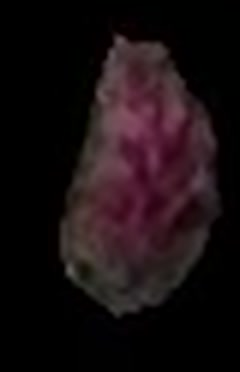
\includegraphics[width=0.21\linewidth]{rainier/motion-54.jpg}\hfill
      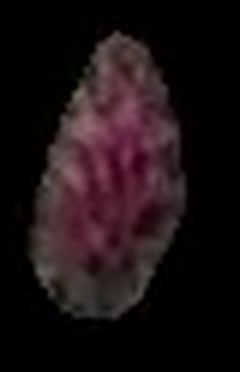
\includegraphics[width=0.21\linewidth]{rainier/motion-82.jpg}\hfill
      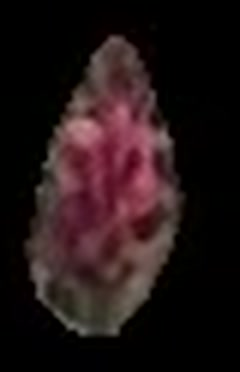
\includegraphics[width=0.21\linewidth]{rainier/motion-120.jpg}\\[0.3em]
      {\scriptsize\color{muted} One tracked flower: \SI{0}{\second},
       \SI{1.2}{\second}, \SI{2.3}{\second}, \SI{3.9}{\second}}
    \end{column}
    \begin{column}{0.58\textwidth}
      \scriptsize
      \begin{itemize}\setlength\itemsep{0.6em}
        \item LTX-2 generates a short video with the camera locked off, so centroid
              drift is the object moving.
        \item Drift under $60\%$ of its own bounding-box diagonal means anchored:
              it gets a sway amplitude and frequency, and a three-bone rig.
        \item Anything drifting further is a rigid body --- velocity and
              acceleration handed to the physics engine.
        \item One scene-global wind field, so a gust crosses the meadow and
              everything in its path responds in turn.
      \end{itemize}
    \end{column}
  \end{columns}
\end{frame}

% 17 -------------------------------------------------------------------------
\begin{frame}{Three captures, chosen to break different assumptions}
  \kicker{results}
  \begin{columns}[T]
    \begin{column}{0.32\textwidth}\centering
      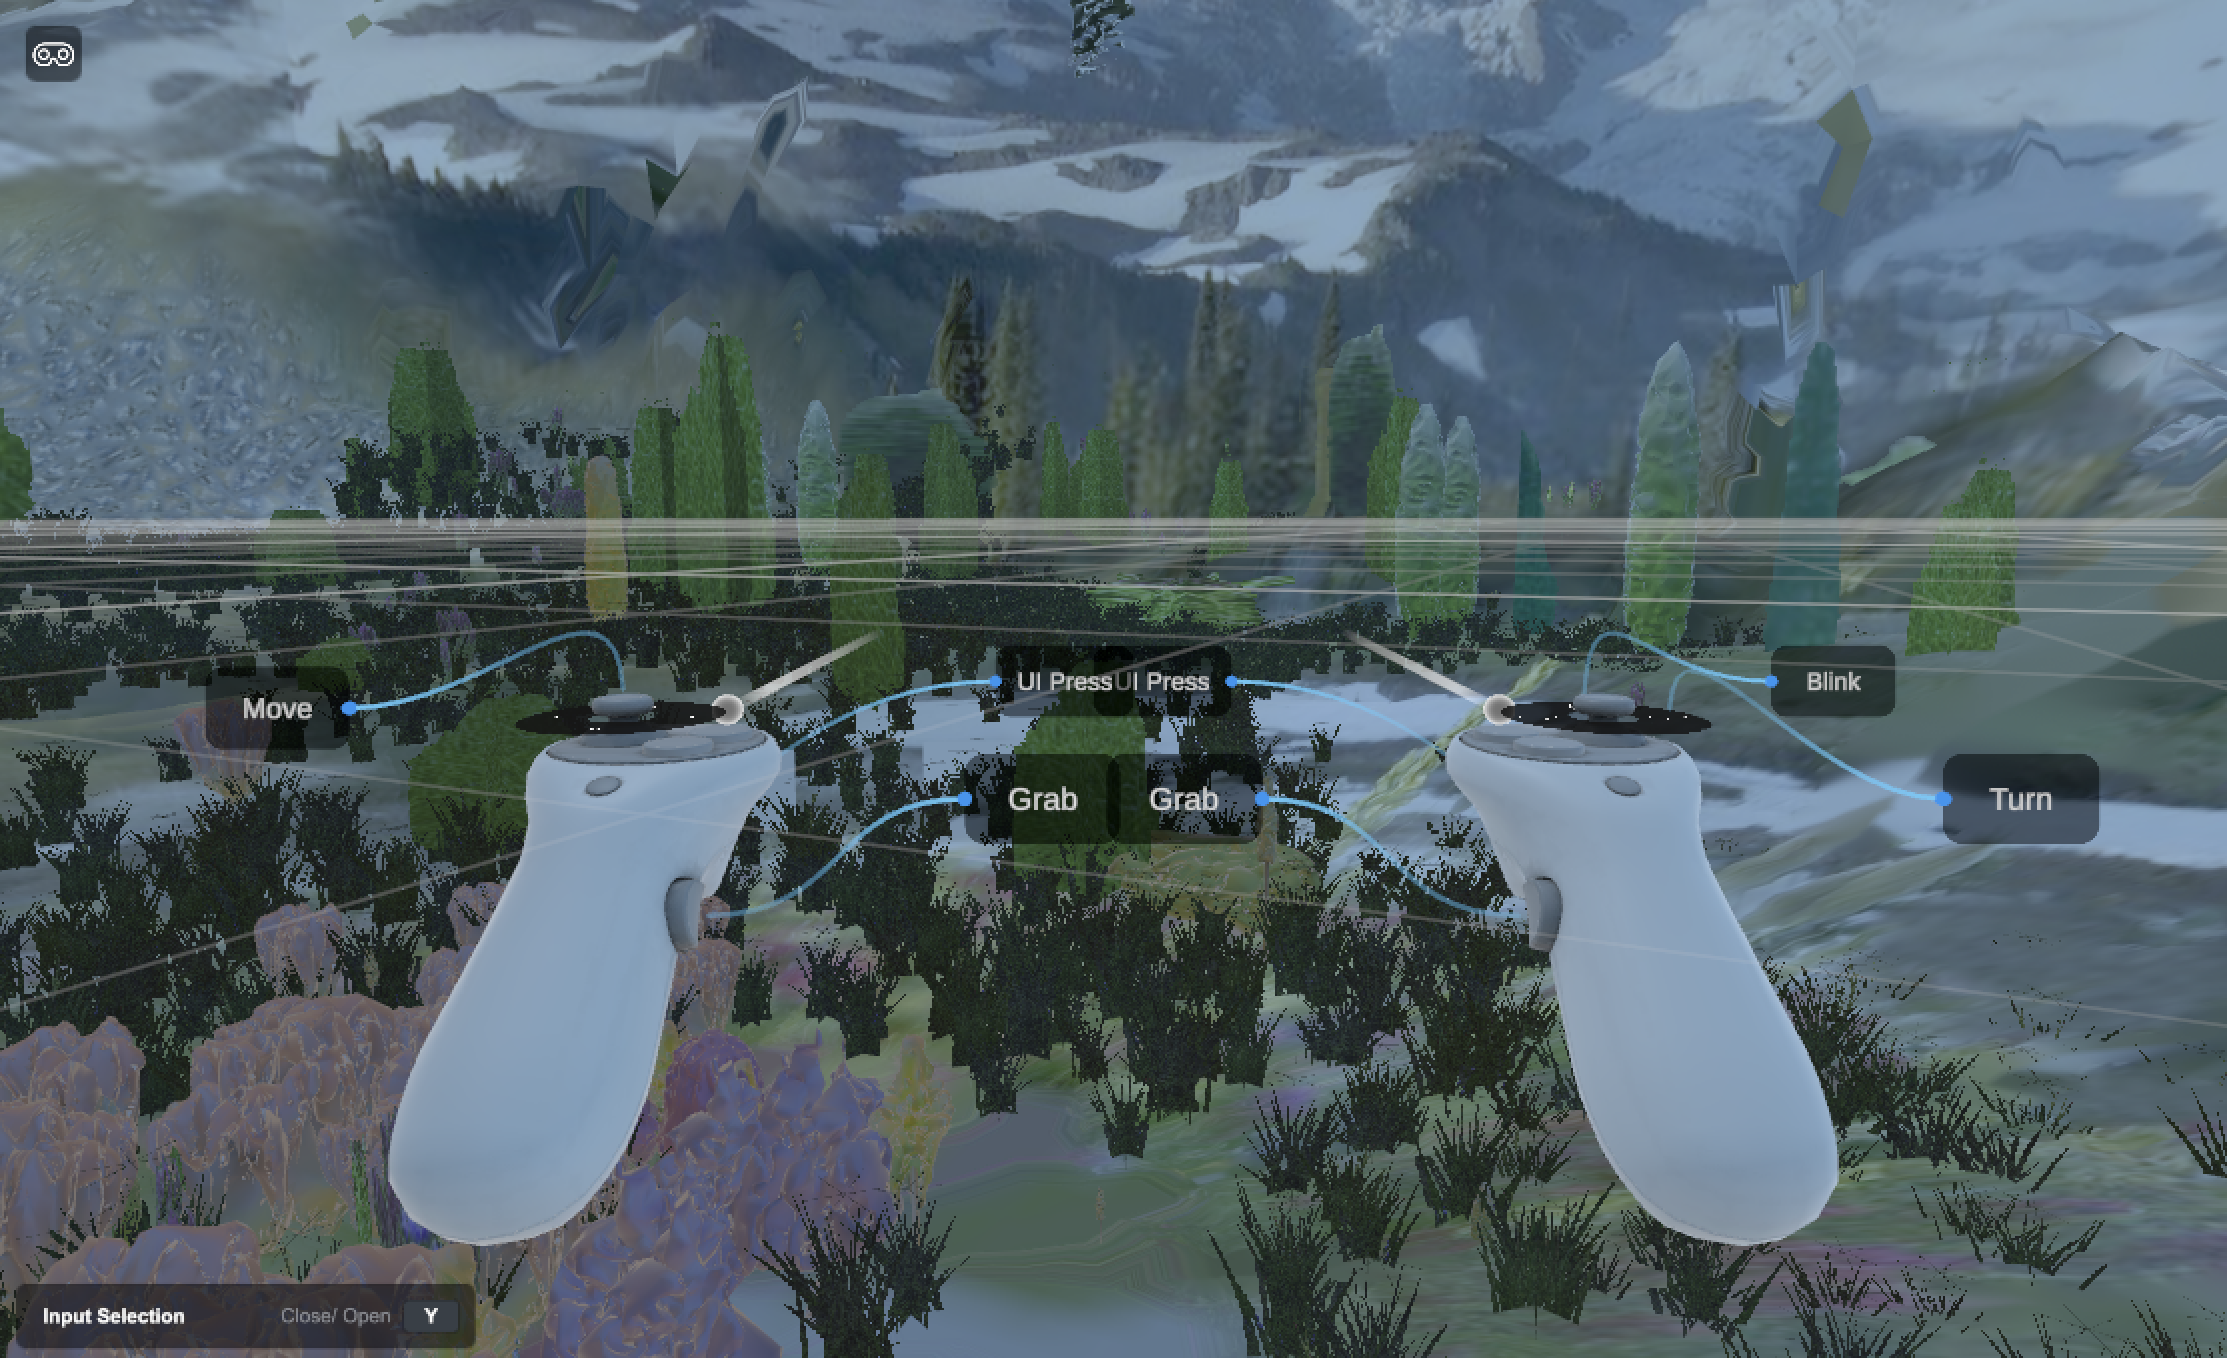
\includegraphics[width=\linewidth]{rainier-scene.png}\\[0.25em]
      {\scriptsize\color{muted} Mount Rainier --- alpine meadow}
    \end{column}
    \begin{column}{0.32\textwidth}\centering
      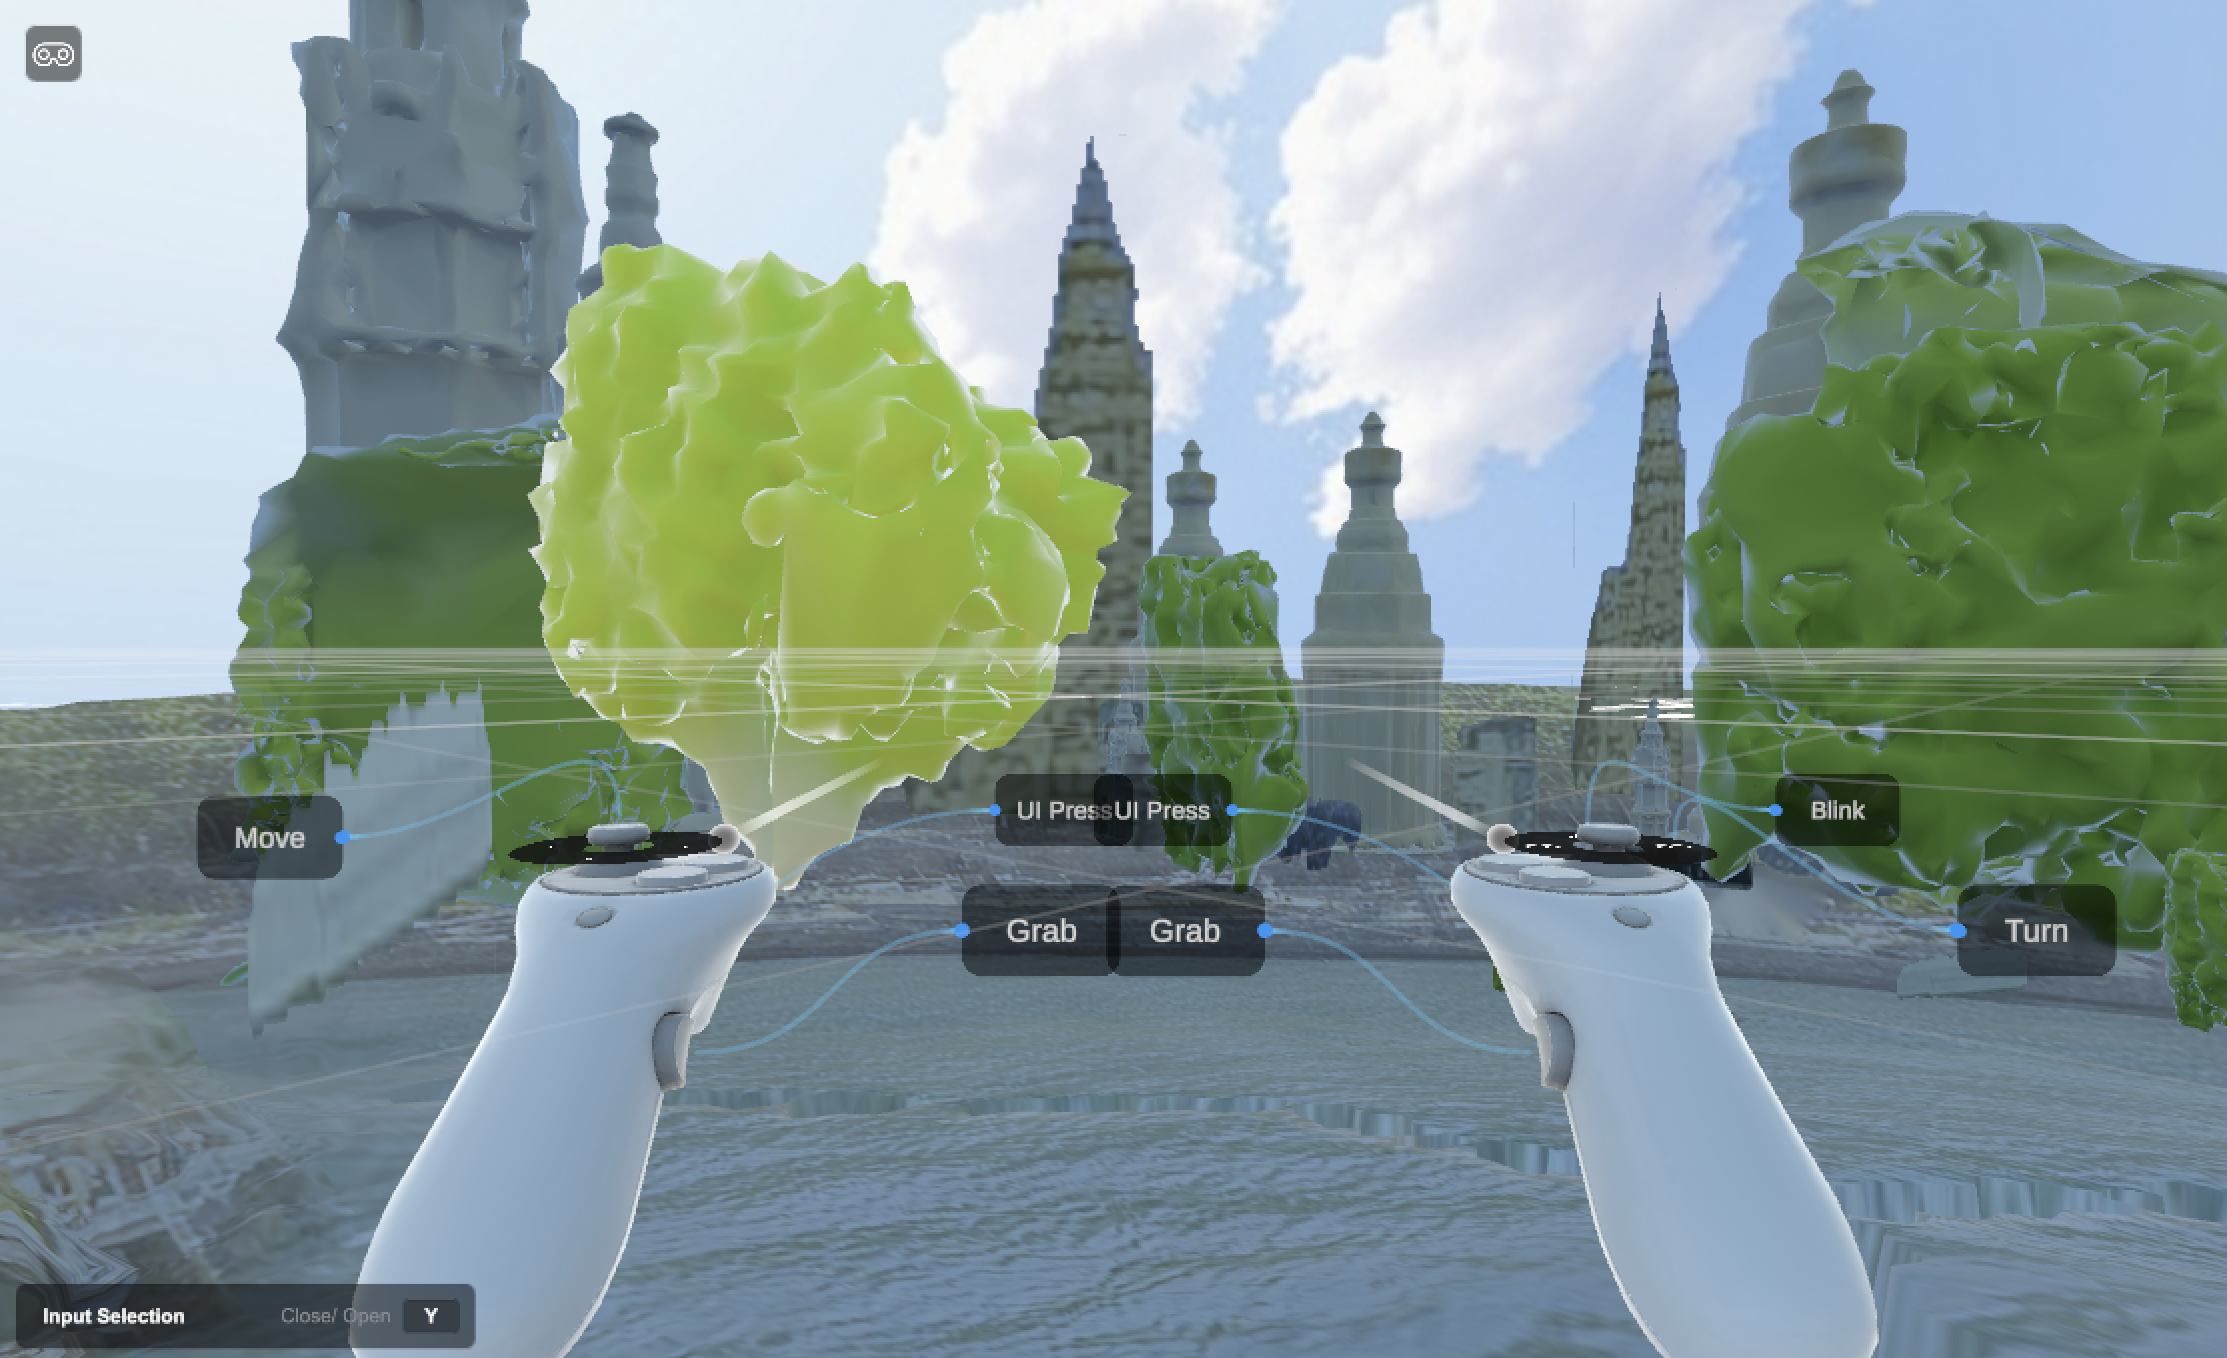
\includegraphics[width=\linewidth]{paris-scene.png}\\[0.25em]
      {\scriptsize\color{muted} Paris --- flat urban river scene}
    \end{column}
    \begin{column}{0.32\textwidth}\centering
      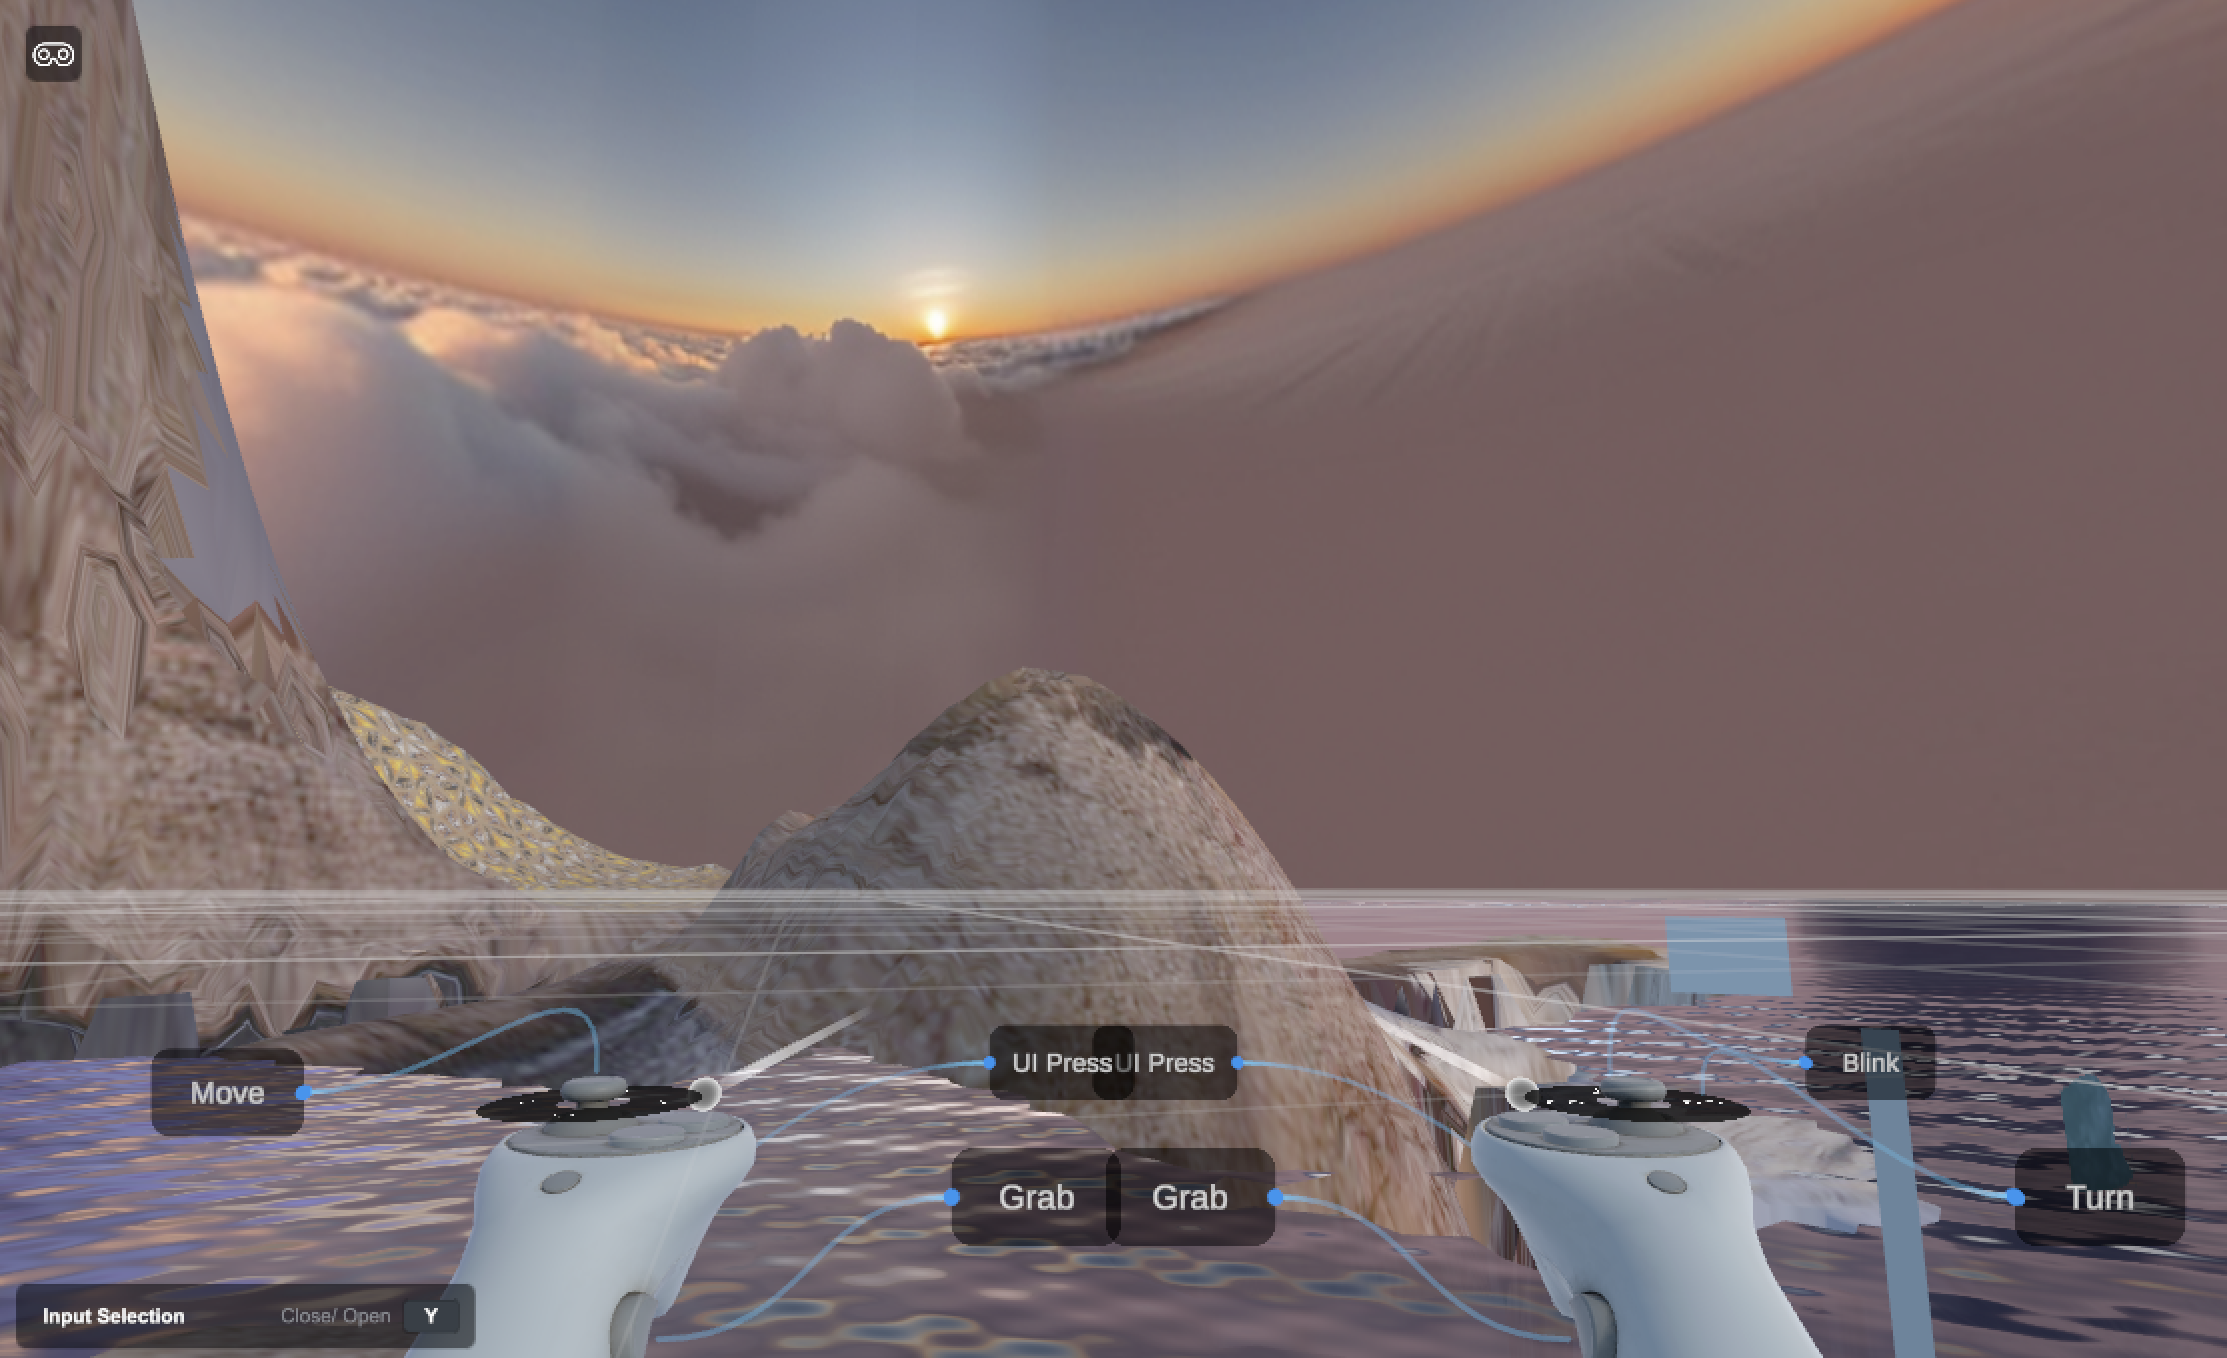
\includegraphics[width=\linewidth]{sharkfin-scene.png}\\[0.25em]
      {\scriptsize\color{muted} Shark Fin Cove --- coastal cliffs}
    \end{column}
  \end{columns}
  \vspace{0.9em}
  \par\raggedright\small
  No ground-truth 3D exists for any of them, so evaluation is diagnostic:
  instrument the pipeline, measure intermediates against what the scene
  demonstrably contains, localize defects to stages.
\end{frame}

% 18 -------------------------------------------------------------------------
\begin{frame}{Every failure localized to an assumption, not a model}
  \kicker{results}
  \footnotesize
  \begin{tabular}{@{}p{4.1cm}p{8.4cm}@{}}
    \lead{Skyline read as landform} & Paris: $0\%$ of horizon columns type terrain, against $98\%$ and $100\%$ elsewhere \\[0.45em]
    \lead{Confident misclassification} & Shark Fin: 49 detections at median confidence $0.95$, almost all rock texture \\[0.45em]
    \lead{Thin vegetation} & SAM~3D returns aspect $3.50{:}1$ against detections at $0.12{:}1$ --- a $28\times$ disagreement \\[0.45em]
    \lead{Water follows terrain} & \SI{11872}{\meter\squared} of sea spanning \SI{73.5}{\meter} in elevation --- the ocean draped up the cliffs \\[0.45em]
    \lead{Far-field texture} & $67.8\%$ of Shark Fin's terrain exceeds \SI{0.5}{\meter} per texel, against $20.9\%$ for Rainier \\
  \end{tabular}
  \vspace{1.0em}
  \par\small
  \flag{Each was fixed by making its premise testable from evidence the pipeline
  already computes} \quietx{--- not by tuning a threshold or swapping a model, and
  measured on every capture rather than only the one that broke.}
\end{frame}

% 19 -------------------------------------------------------------------------
\begin{frame}{The transferable result is methodological}
  \kicker{what we learned}
  \small
  Into Frame mixes learned models and classical graphics roughly two-to-one by
  stage count. Neither part would produce this output alone.
  \vspace{0.9em}
  \begin{columns}[T]
    \begin{column}{0.47\textwidth}
      {\color{accent}\bfseries\scriptsize GENERATIVE MODELS}\par\vspace{0.35em}
      \scriptsize Make the problem tractable at all. Five sixths of the sphere and
      the ground behind every object are never observed, and no classical reasoning
      recovers content absent from the input.\par\vspace{0.5em}
      \lead{They answer \emph{what is there}.}
    \end{column}
    \begin{column}{0.47\textwidth}
      {\color{accent}\bfseries\scriptsize CLASSICAL GRAPHICS}\par\vspace{0.35em}
      \scriptsize Supply the structure. A harmonic solve that never modifies
      measured ground, fluvial incision, point-process synthesis, pattern
      texturing, a rig driven by a shared wind field.\par\vspace{0.5em}
      \lead{They decide \emph{how it behaves}.}
    \end{column}
  \end{columns}
  \vspace{1.1em}
  \par\footnotesize\color{muted}
  Of 38 active stages, 12 use no learned model at all --- and those are
  disproportionately the ones that produce the scene's physical behavior.
\end{frame}

% 20 -------------------------------------------------------------------------
\begin{frame}{Where this leaves us}
  \kicker{conclusions \& future work}
  \begin{columns}[T]
    \begin{column}{0.50\textwidth}
      \small
      \begin{itemize}\setlength\itemsep{0.6em}
        \item A single photograph becomes an interactive environment with terrain,
              objects, ground cover, water and lighting as distinct physical
              components.
        \item The decomposition buys the depth of the result --- each component
              behaves according to its role.
        \item Remaining failures are assumptions that held for outdoor natural
              landscapes and did not extrapolate.
      \end{itemize}
    \end{column}
    \begin{column}{0.46\textwidth}
      {\color{accent}\bfseries\scriptsize FUTURE WORK}\par\vspace{0.4em}
      \scriptsize
      \begin{itemize}\setlength\itemsep{0.35em}
        \item Explicit scene classification, consumed by every stage embedding an
              implicit assumption
        \item Confidence propagation, so the system can report where it is guessing
        \item Species-aware reconstruction for thin structures
        \item Joint refinement across depth, geometry and placement
        \item Perceptual evaluation in the headset
        \item Spatialized audio and richer interaction
      \end{itemize}
    \end{column}
  \end{columns}
  \vspace{1.0em}
  \par\centering\small
  \lead{The boundaries are legible and measurable} --- addressing them means making
  implicit commitments explicit, rather than waiting for better models.
\end{frame}

\end{document}
